%%%%%%%%%%%%%%%%%%%%%%%%%%%%%%%%%%%%%%%%%
% Short Sectioned Assignment LaTeX Template Version 1.0 (5/5/12)
% This template has been downloaded from: http://www.LaTeXTemplates.com
% Original author:  Frits Wenneker (http://www.howtotex.com)
% License: CC BY-NC-SA 3.0 (http://creativecommons.org/licenses/by-nc-sa/3.0/)
%%%%%%%%%%%%%%%%%%%%%%%%%%%%%%%%%%%%%%%%%

%----------------------------------------------------------------------------------------
%	PACKAGES AND OTHER DOCUMENT CONFIGURATIONS
%----------------------------------------------------------------------------------------

\documentclass[paper=a4, fontsize=11pt]{scrartcl} % A4 paper and 11pt font size

% ---- Entrada y salida de texto -----
\usepackage{listings}
\usepackage[T1]{fontenc} % Use 8-bit encoding that has 256 glyphs
\usepackage[utf8]{inputenc}
%\usepackage{fourier} % Use the Adobe Utopia font for the document - comment this line to return to the LaTeX default

% ---- Idioma --------

\usepackage{svg}
\usepackage{amsmath}
\usepackage[spanish, es-tabla]{babel} % Selecciona el español para palabras introducidas automáticamente, p.ej. "septiembre" en la fecha y especifica que se use la palabra Tabla en vez de Cuadro

% ---- Otros paquetes ----

\usepackage{url} % ,href} %para incluir URLs e hipervínculos dentro del texto (aunque hay que instalar href)
\usepackage{amsmath,amsfonts,amsthm} % Math packages
%\usepackage{graphics,graphicx, floatrow} %para incluir imágenes y notas en las imágenes
\usepackage{graphics,graphicx, float} %para incluir imágenes y colocarlas

% Para hacer tablas comlejas
%\usepackage{multirow}
%\usepackage{threeparttable}

%\usepackage{sectsty} % Allows customizing section commands
%\allsectionsfont{\centering \normalfont\scshape} % Make all sections centered, the default font and small caps

\usepackage{fancyhdr} % Custom headers and footers
\pagestyle{fancyplain} % Makes all pages in the document conform to the custom headers and footers
\fancyhead{} % No page header - if you want one, create it in the same way as the footers below
\fancyfoot[L]{} % Empty left footer
\fancyfoot[C]{} % Empty center footer
\fancyfoot[R]{\thepage} % Page numbering for right footer
\renewcommand{\headrulewidth}{0pt} % Remove header underlines
\renewcommand{\footrulewidth}{0pt} % Remove footer underlines
\setlength{\headheight}{13.6pt} % Customize the height of the header

\numberwithin{equation}{section} % Number equations within sections (i.e. 1.1, 1.2, 2.1, 2.2 instead of 1, 2, 3, 4)
\numberwithin{figure}{section} % Number figures within sections (i.e. 1.1, 1.2, 2.1, 2.2 instead of 1, 2, 3, 4)
\numberwithin{table}{section} % Number tables within sections (i.e. 1.1, 1.2, 2.1, 2.2 instead of 1, 2, 3, 4)

\setlength\parindent{0pt} % Removes all indentation from paragraphs - comment this line for an assignment with lots of text

\newcommand{\horrule}[1]{\rule{\linewidth}{#1}} % Create horizontal rule command with 1 argument of height


%----------------------------------------------------------------------------------------
%	TÍTULO Y DATOS DEL ALUMNO
%----------------------------------------------------------------------------------------

\title{	
\normalfont \normalsize 
\textsc{\textbf{Ingeniería de Servidores (2016-2017)} \\ Grado en Ingeniería Informática \\ Universidad de Granada} \\ [25pt] % Your university, school and/or department name(s)
\horrule{0.5pt} \\[0.4cm] % Thin top horizontal rule
\huge Memoria Práctica 1 \\ % The assignment title
\horrule{2pt} \\[0.5cm] % Thick bottom horizontal rule
\begin{figure*}[!ht]
	\begin{center}
		
\includegraphics[width=0.7\textwidth]{imagenes/escudo-de-la-universidad-de-granada}
	\end{center}
\end{figure*}
}

\author{Iván Rodríguez Millán} % Nombre y apellidos

\date{\normalsize\today} % Incluye la fecha actual

%----------------------------------------------------------------------------------------
% DOCUMENTO
%----------------------------------------------------------------------------------------


\begin{document}

\maketitle % Muestra el Título
\thispagestyle{empty} % Ns quita la numeración de página

\newpage %inserta un salto de página

\tableofcontents % para generar el índice de contenidos

\listoffigures

\listoftables

\newpage

%----------------------------------------------------------------------------------------
%	Cuestión 1
%----------------------------------------------------------------------------------------

\section{?`Que modos y/o tipos de virtualización existen?}

\subsection{Respuesta:}
Tipos de virtualización descritos por la empresa VMWare \cite{cuestion1} :
\begin{itemize}
	\item Virtualización de servidor: Ejecución de varios sistemas operativos en un mismo servidor físico.
	\item Virtualización de escritorio: Escritorios almacenados en un servidor, en vez de en el ordenador desde el que se trabaja.
	\item Virtualización de redes: Proporciona instancias virtuales de redes físicas, dividiendo el ancho de banda en diferentes canales.
\end{itemize}

%----------------------------------------------------------------------------------------
%	Cuestión 2
%----------------------------------------------------------------------------------------

\section{Muestre los precios y características de varios proveedores de VPS (Virtual Private Server) y compare con el precio de servidores dedicados (administrados y no administrados). Comente diferencias.}

\subsection{Respuesta:}

\begin{savenotes}
    \begin{table}[H]
	\centering
	\begin{tabular}{|c|c|c|c|c|l|}
	\hline
	\textbf{ Proveedor} & \textbf{núcleos} & \textbf{Memoria} & \textbf{Disco} & \textbf{Precio(mes)} & \textbf{SO} \\
	\hline
	Inmotion Hosting\cite{cuestion2A} & Ilimitados\footnote{La empresa no pone un límite, pero si llega el momento en que se hace demasiado uso de CPU y eso afecta a otros usuarios variarán el plan} & 6 GB & 130 GB & \$49,99 & centOS  \\
	\hline
	1\&1 \cite{cuestion2B} & 4 & 8 GB & 160 GB SSD & 19,99\euro & Linux	 \\
	\hline
	Arvixe\cite{cuestion2C} & 4 & 1.5 GB & 50 GB & \$40 & centOS \\
	\hline
	\end{tabular} 
	\caption{Precios de Proveedores de VPS} \label{tab:tablaProvVPS}
	\end{table}
    \end{savenotes}
    
\begin{table}[H]
\centering
\begin{tabular}{|l|c|c|c|c|l|}
\hline
\textbf{ Proveedor} & \textbf{núcleos} & \textbf{Memoria} & \textbf{Disco} & \textbf{Precio(mes)} & \textbf{SO} \\
\hline
Inmotion Hosting\cite{cuestion2D} & 4 & 8 GB & 1 TB & \$99,99 & centOS \\
\hline
1\&1\cite{cuestion2E} & 12 & 64 GB & 4 TB & 64,99\euro & Linux	 \\
\hline
Arvixe\cite{cuestion2F} & 4 & 4 GB & 128 GB SSD  & \$128,70 & Linux \\
\hline
\end{tabular}  
\caption{Precios de Proveedores de servidores dedicados} \label{tab:tablaProvSD}
\end{table}

Como bien se puede apreciar en las tablas anteriores el precio de un servidor virtual privado con respecto a un servidor dedicado es bastante menor. Ocurre en gran parte porque en realidad en un VPS compartes un gran número de recursos del servidor físico, mientras que en un servidor dedicado el uso está reservado exclusivamente para el usuario.\cite{VPSvsDedInmotion}

%----------------------------------------------------------------------------------------
%	Cuestión 3
%----------------------------------------------------------------------------------------
\section{Enumere y explique brevemente al menos tres de las innovaciones en Windows Server 2016 y 2012 R2 respecto a 2008 R2.
	?`Què es Windows Server 2016 nano?}
\subsection{Respuesta a):}

\begin{enumerate}
\item Virtualización de Active Directory: Desde Windows Server 2012 R2, se ha mejorado la compatibilidad con la virtualización de controladores de dominio, introduciendo recursos seguros para la virtualización.\cite{cuestion3Aa}
\item VHDX compartido: Otra mejora lograda a partir de Windows Server 2012 R2 fue la de poder compartir archivos(VHDX) de disco duro virtual con varias máquinas virtuales.\cite{cuestion3Ab}
\item El health service (servicio de estado) es una nueva herramienta en Windows server 2016, que facilita la monitorización, las operaciones y el mantenimiento del almacenamiento de espacio directo. Viene habilitado por defecto. Esta característica reduce el trabajo para obtener información sobre el rendimiento en vivo. Incluye la inteligencia necesaria para determinar la causa que provocó un fallo y prestar ayuda.\cite{DifWS2016}
\item Para mejorar la seguridad, WS 2016 incorpora el blindado de máquinas virtuales, que tiene la capacidad de ofrecer un entorno en donde se refuerza la seguridad. La máquina virtual blindada se cifra usando BitLocker. \cite{DifWS2016}
\end{enumerate}
\subsection{Respuesta b):}

Es un sistema operativo de administración remota optimizado para private clouds y datacenters. Es similar a Windows Server en modo Server Core, pero menor pues no cuenta con inicio de sesión local y solo soporta aplicaciones y herramientas de 64-bit.
Requiere bastante menos espacio de disco, es significativamente más rápido y requiere muchas menos actualizaciones con lo que acarrea tener que reiniciar menos el servidor. Además el reinicio es más rápido.
Está pensado para servidores de un tamaño reducido, desprovisto de funciones en este contexto innecesarios y pensado para su administración remota.\cite{cuestion3B}

%----------------------------------------------------------------------------------------
%	Cuestión 4
%----------------------------------------------------------------------------------------
\newpage
\section{?`Qué son los productos MAAS y Landscape ofrecidos por Canonical(empresa que desarrolla Ubuntu)?}
\subsection{Respuesta:}

\begin{itemize}
	\item MAAS: Es una herramienta de aprovisionamiento para servidores, como indica su nombre Metal as a Service(Metal como un servicio), pretende ayudar a trabajar con servidores físicos para actuar con los beneficios del servicio en nube. MAAS hace muy fácil configurar el hardware en el que queremos desplegar servicios que necesitan escalar de forma dinámica. Así convierte el servidor en un recurso elástico similar a una nube.\cite{cuestion4A}
	\item Landscape: Herramienta para administrar equipos con Ubuntu de forma centralizada, destinado para empresas con muchos equipos Ubuntu.
		Permite la monitorización de los equipos, así como poder
		recoger información en tiempo real. También se puede controlar
		temas como actualizaciones(aceptarlas o ponerlas en espera, e
		incluso poder volver atrás),	automatizar las tareas del día a
		día, etc.\cite{LandscapeDocumentation} \\
		Canonical asegura ``ahorrar tiempo y mejorar la
		seguridad''.\cite{cuestion4B}
\end{itemize}

%----------------------------------------------------------------------------------------
%	Cuestión 5
%----------------------------------------------------------------------------------------
\section{?`Qué relación tiene esta distribución con Red Hat y con el proyecto Fedora?}
\subsection{Respuesta:}
CentOS es un sistema operativo de código libre y abierto a cualquier persona que desee utilizarlo. Es una distribución derivada de los paquetes liberados por Red Hat, hoy en día está construida con la mayor parte del código base de Red Hat Enterprise Linux. Con esta colaboración de Red Hat, CentOS puede cubrir mejor las necesidades de los miembros de la comunidad de código abierto. \cite{cuestion5BB}
	\\
	A su vez el proyecto Fedora mantiene una relación de patrocinio con Red Hat, que invierte recursos para la colaboración llevando las innovaciones más actuales para que se consoliden, actuando Fedora como incubadora de nuevas tecnologías que más tarde podrán ser integradas en Red Hat.\cite{cuestion5C}
	
%----------------------------------------------------------------------------------------
%	Cuestión 6
%----------------------------------------------------------------------------------------
\section{?`Qué diferencias hay entre RAID mediante SW y mediante HW?}
\subsection{Respuesta:}
El RAID por Hardware se monta gracias a controladoras dedicadas a gestionar el RAID por sí mismas. \cite{RAIDRed_Hat} \\
Según Dakel(Empresa): la controladora crea una capa de abstracción entre el sistema RAID y la propia máquina, evitando que el sistema consuma recursos atendiendo y gestionando el RAID, y además permite optimizar el acceso a disco. \cite{cuestion6A}\newpage
El RAID por Software permite incrementar el rendimiento y la fiabilidad de discos sin necesidad del uso de controladoras y RAID caros. Permite combinar particiones y redireccionarlas como un único dispositivo RAID. RAID por software ofrece una solución más barata ya que no son necesarias las tarjetas del controlador de disco, que suelen ser caros.\cite{RAIDSWGentoo}\cite{RAIDRed_Hat}

%----------------------------------------------------------------------------------------
%	Cuestión 7
%----------------------------------------------------------------------------------------
\section{?`Qué es LVM?.?`Qué ventaja tiene para un servidor de gama baja?.Si va a tener un servidor Web, ?`Le daría un tamaño grande o pequeño a /var?}
\subsection{Respuesta a):}
 LVM son las iniciales de logical volume manager(gestor de volúmenes lógicos), es una forma de abstraer los volúmenes lógicos del soporte físico ofreciendo una mayor flexibilidad, LVM nos permite modificar un volumen lógico de forma transparente a las aplicaciones.\cite{ManualDebian}\\
 Básicamente LVM controla los recursos de disco relacionando los datos entre una vista lógica más simple y flexible, y los discos físicos reales.\cite{IBMLVM}
 \subsection{Respuesta b):}
 El uso de volúmenes lógicos sobre un servidor de gama baja tiene las siguientes ventajas:\cite{RedHatVentajasLVM}
 \begin{itemize}
 	\item Las agrupaciones de almacenamiento son de tamaño variable, ya que puedes ampliar o reducir el tamaño de los volúmenes lógicos, de una manera sencilla, sin formatear y particionar.
 	\item Permite la asignación de datos en linea, que no es más que poder mover datos mientras el sistema está activo, y así los datos pueden ser reorganizados en los discos.
 	\item Los volúmenes lógicos pueden ser manejados a su vez desde grupos  definidos por el propio usuario.
 	\item Se pueden implementar volúmenes espejo.
 \end{itemize}
 \subsection{Respuesta c):}
 La carpeta /var en servidores web suele ir separado del directorio raíz por varios aspectos:
 \begin{itemize}
 	\item Para reducir el tiempo de acceso puesto que aquí se alojan bases de datos y archivos a los que nos interesan tener buenos tiempos de lectura y escritura.
 	\item Para mayor seguridad podríamos pensar en ubicarlo en discos que dispongan de mayores medidas de seguridad por la  condición crítica que pueden llegar a tener los archivos.
 	\item Y por ultimo y más relevante para nuestro estudio, en este directorio los archivos suelen experimentar un crecimiento muy rápido y puede llegar a descontrolarse, dejando nuestro sistema sin espacio. Esto ocurre porque aquí residen datos variables tales como: artículos de noticias, e-mails, páginas webs, caché APT, etc.\cite{cuestion7C}
 	\end{itemize}
 	Por esto último en particular sería bastante lógico darle un tamaño grande cuándo se tiene un servidor web.

%----------------------------------------------------------------------------------------
%	Cuestión 8
%----------------------------------------------------------------------------------------
\section{?`Debemos cifrar también el volumen que contiene el espacio para swap?. ?`Y el volumen en el que montaremos /boot?}
\subsection{Respuesta a):}
En el caso del volumen que contiene el espacio para swap(área de intercambio) se debería cifrar, por el siguiente motivo expuesto en el manual de Debian:
Imaginemos que tenemos una partición cifrada, en este caso la clave se almacena en la memoria (RAM), si se obtiene esta clave, se puede acceder a los datos, y esto puede ocurrir fácilmente ya que al hibernar se almacenan los contenidos de la RAM en la partición SWAP, y si esta partición no está cifrada se puede acceder a la clave. Por ejemplo en instalaciones con Debian, el propio instalador advertirá al usuario si intenta cifrar una partición cuando el SWAP no esté cifrado.\cite{ManualInstalacionDebian}
\subsection{Respuesta b):}
Según el manual GNU GRUB 2.00 \cite{cuestion8BB}, el GRUB no es capaz de leer desde dispositivos encriptados. Luego atendiendo al propio manual, la respuesta sería no cifrar el volumen /boot.

%----------------------------------------------------------------------------------------
%	Cuestión 9
%----------------------------------------------------------------------------------------
\section{Imagine que tiene un disco híbrido con tecnología SSD, ?`Qué puntos de montaje ubicaría en este?. Justifique qué tipo de sistema de archivos usaría para tener un servidor de streaming.}
\subsection{Respuesta a):}
En el caso de tener la posibilidad de contar con un disco SSD los puntos de montaje que en mi opinión deberían estar son:
El /boot, para agilizar el arranque del sistema, y la raíz (/) para mejorar la ejecución de las aplicaciones que vayan a correr en la máquina, dejando fuera el /home.
Cabe decir que no es bueno someter a un dispositivo SSD a muchas escrituras.
\newpage
\subsection{Respuesta b):}
Para un servidor streaming escojo la opción de Ext4 en primer lugar por contar con pre-allocation(pre-asignación), que permite la reserva de espacio en disco para un fichero. Ahora el espacio quedará garantizado y con casi total seguridad será contiguo. En segundo lugar se mejora la fragmentación interna al elegir bloques contiguos con la característica de asignación de bloques múltiples. Y no hay que olvidarse de que el sistema de archivos ext4 cuenta con el famoso Journaling(registro diario) para tener el sistema de archivos en un estado coherente. 
	Y por último cabe decir que el tamaño máximo de archivo que admite es de 16 TiB, estando por encima de ext2 y ext4, entre otros.
\cite{RedHatSFext4}

%----------------------------------------------------------------------------------------
%	Cuestión 10
%----------------------------------------------------------------------------------------
\section{Muestre cómo ha quedado el disco particionado una vez el sistema está instalado y ha iniciado sesión.(comando: lsblk)}
\subsection{Respuesta:}
\begin{figure}[H]
	\begin{center}
		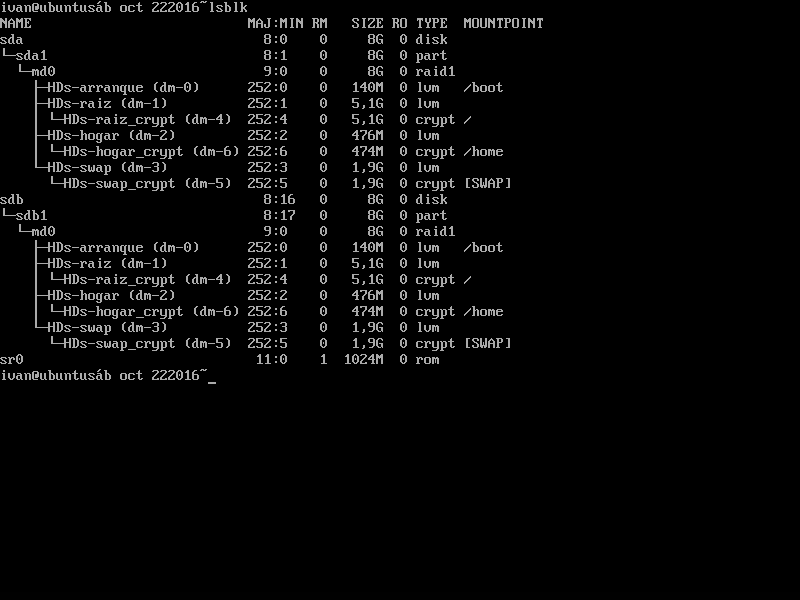
\includegraphics[width=0.7\textwidth]{Imagenes/Disco-final-particionado}
		\caption{Particionado final del sistema} \label{fig:figura1}
	\end{center}
\end{figure}

\newpage
%----------------------------------------------------------------------------------------
%	Cuestión 11
%----------------------------------------------------------------------------------------
\section{a)?`Cómo ha hecho el disco 2 ''arrancable'' ? b)?`Qué hace el comando grub-install?}
\subsection{Respuesta a):}
En primer lugar instalamos con el comando grub-install el grub en el disco 2:
\begin{figure}[H]
	\begin{center}
		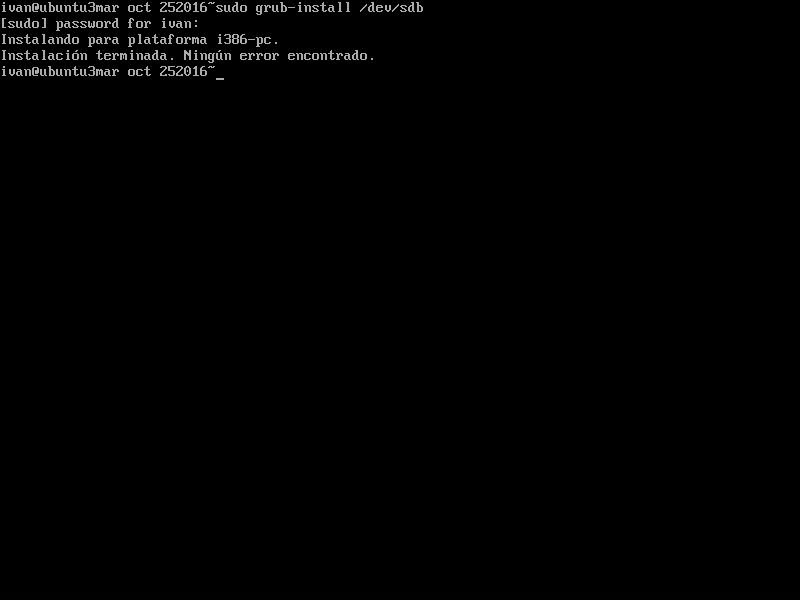
\includegraphics[width=0.7\textwidth]{Imagenes/01_Instalando_Grub}
		\caption{Instalación Grub en disco 2.} \label{fig:figura1}
	\end{center}
\end{figure}	
Cuando terminemos con la instalación del Grub, salimos a VirtualBox y en la parte de almacenamiento eliminamos la partición 1.
\begin{figure}[H]
	\begin{center}	
		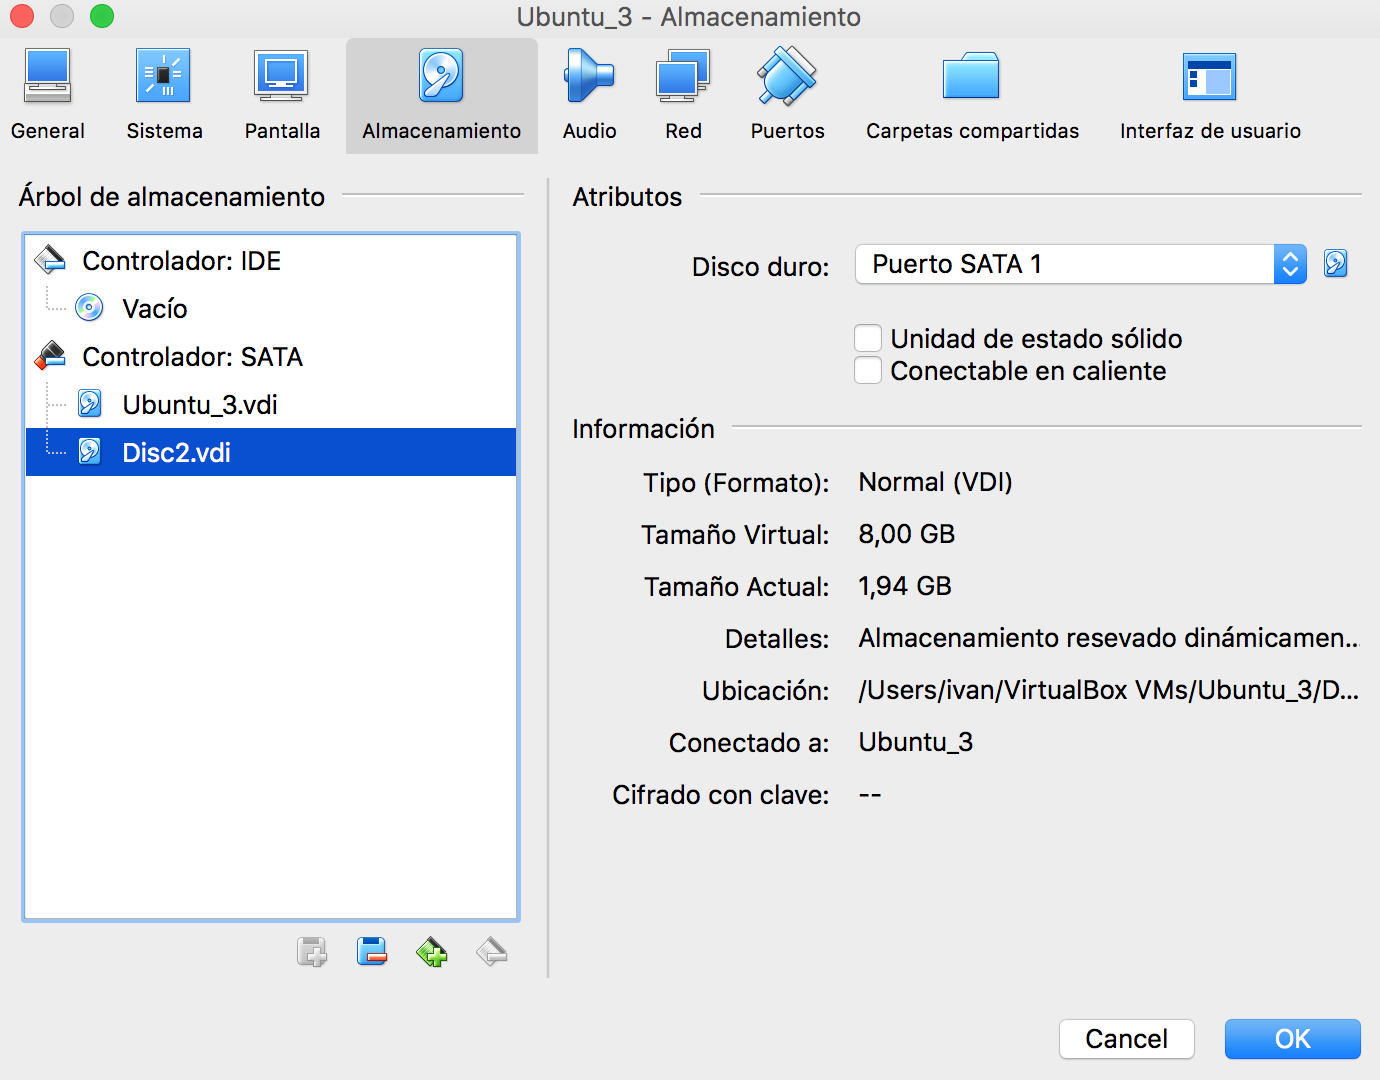
\includegraphics[width=0.7\textwidth]{Imagenes/02_Eliminando_particion_1}
		\caption{Eliminando disco 1 desde VirtualBox.} \label{fig:figura2}
	\end{center}
\end{figure}
Una vez eliminada la partición 1, volvemos a arrancar la máquina virtual.
\begin{figure}[H]
	\begin{center}
		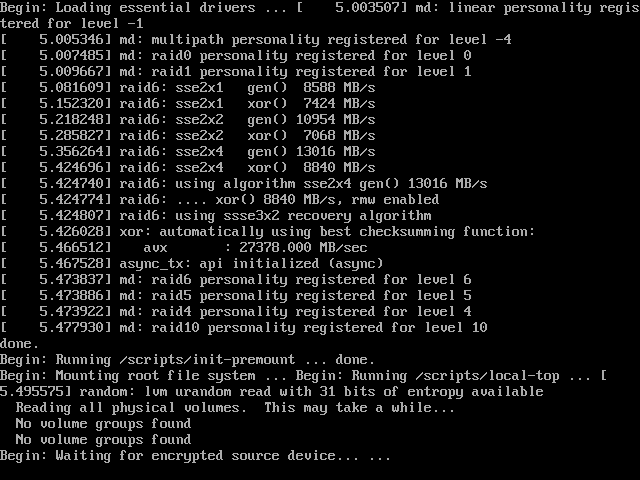
\includegraphics[width=0.7\textwidth]{Imagenes/03_Entrando1}
		\caption{Entrando de nuevo una vez eliminada la partición 1.} \label{fig:figura3}
		\end{center}
\end{figure}
\newpage
Lo que debemos hacer es esperar hasta que nos aparezca initramfs.
\begin{figure}[H]
	\begin{center}		
		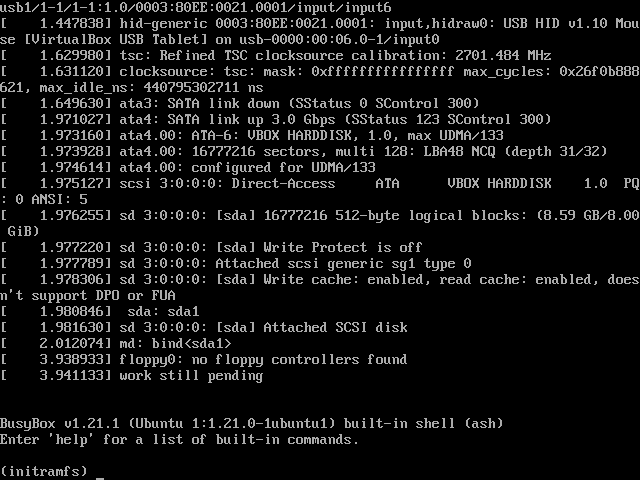
\includegraphics[width=0.7\textwidth]{Imagenes/04_Entrando2}
		\caption{Prompt initramfs.} \label{fig:figura4}
	\end{center}
\end{figure}
Una vez dentro procederemos a arrancar desde el disco 2. En primer lugar visualizamos el estado de los discos y unidades RAID mediante el siguiente comando:
\begin{figure}[H]
	\begin{center}		
		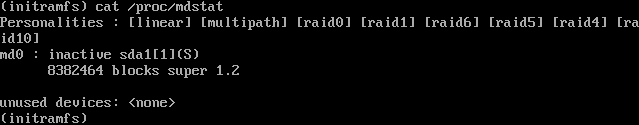
\includegraphics[width=0.7\textwidth]{Imagenes/05_visualizando_actividad}
		\caption{Comprobación del estado del RAID.} \label{fig:figura5}
	\end{center}
\end{figure}
En caso de que el estado del RAID sea el de inactivo, con el siguiente comando lo activamos. \cite{MDADMMAN}
\begin{figure}[H]
	\begin{center}		
		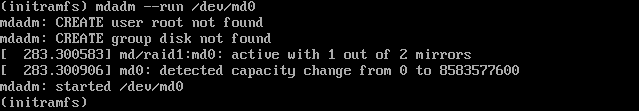
\includegraphics[width=0.7\textwidth]{Imagenes/06_Activando_Particion_2}
		\caption{Puesta en marcha del RAID.} \label{fig:figura6}
	\end{center}
\end{figure}
Una vez hecho este paso, volvemos a comprobar el estado del RAID, que si todo ha ido normal, habrá cambiado a activo.
\begin{figure}[H]
	\begin{center}		
		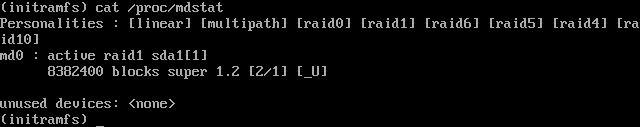
\includegraphics[width=0.7\textwidth]{Imagenes/07_Visualizando_Actividad_raid}
		\caption{Comprobación para ver si el estado del RAID a cambiado a activo.} \label{fig:figura7}
	\end{center}
\end{figure}
Después solamente tendremos que salirnos, y proceder con el desencriptado de las distintas particiones.
\begin{figure}[H]
	\begin{center}		
		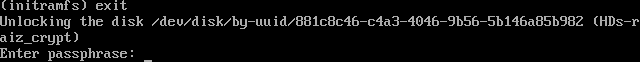
\includegraphics[width=0.7\textwidth]{Imagenes/08_Saliendo_initramfs}
		\caption{Introducción de contraseñas para el desencriptado de las distintas particiones.} \label{fig:figura8}
	\end{center}
\end{figure}
Finalmente se nos pedirá el login y password de usuario, y el proceso habrá finalizado satisfactoriamente.
\begin{figure}[H]
	\begin{center}		
		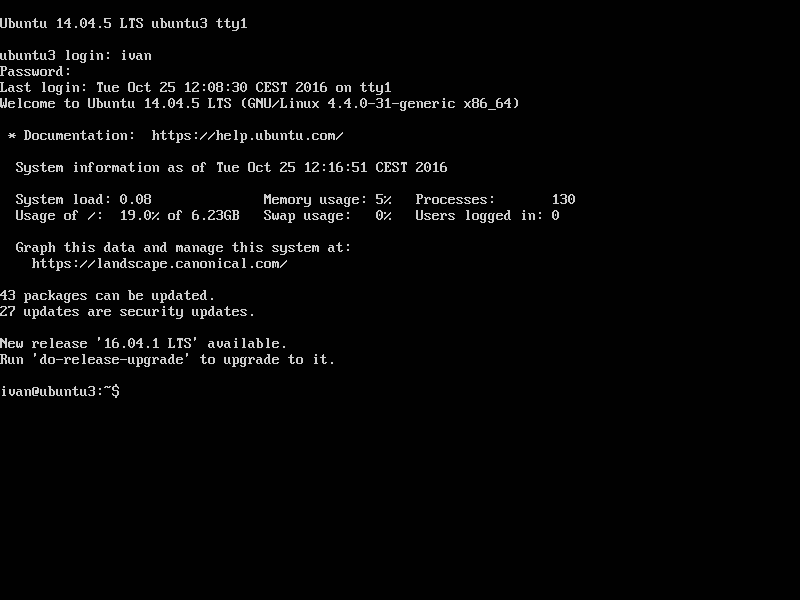
\includegraphics[width=0.7\textwidth]{Imagenes/09_Estado_Final}
		\caption{Introducción del Login y Password de usuario.} \label{fig:figura9}
	\end{center}
\end{figure}

\subsection{Respuesta b):}
El comando grub-install nos permite instalar el GRUB en un dispositivo. El comando debe ir acompañado del nombre del dispositivo en donde se instalará. \cite{cuestion8BB}
%----------------------------------------------------------------------------------------
%	Cuestión 12
%----------------------------------------------------------------------------------------
\section{?`Qué diferencia hay entre Standard y Datacenter?}
\subsection{Respuesta:}
En las ediciones de Windows Server 2012:\\

\begin{itemize}
	\item La edición Datacenter es perfecto para usuarios que quieran tener un entorno de nube privada e híbrido muy virtualizado. Permite la capacidad de albergar una cantidad ilimitada de equipos virtuales. Proporciona todas las características del producto. Microsoft afirma que se tienen instancias limitadas de WS con cada licencia. 
	\cite{MicrosoftDatacenterVSStandard}
	\item Mientras la edición Standard es ideal para los usuarios que quieran tener un entorno físico o ligeramente virtualizado. Con la licencia de 2012 se permite al usuario ejecutar hasta dos instancias virtuales de Windows Server con cada licencia, aparte de proporcionar todas las características de WS Datacenter. El licenciamiento cambió con el lanzamiento de WS 2012 y ahora es el mismo que para la edición Datacenter.\cite{MicrosoftDatacenterVSStandard}

En las ediciones de Windows Server 2016:
\end{itemize}
\begin{figure}[H]
	\begin{center}
		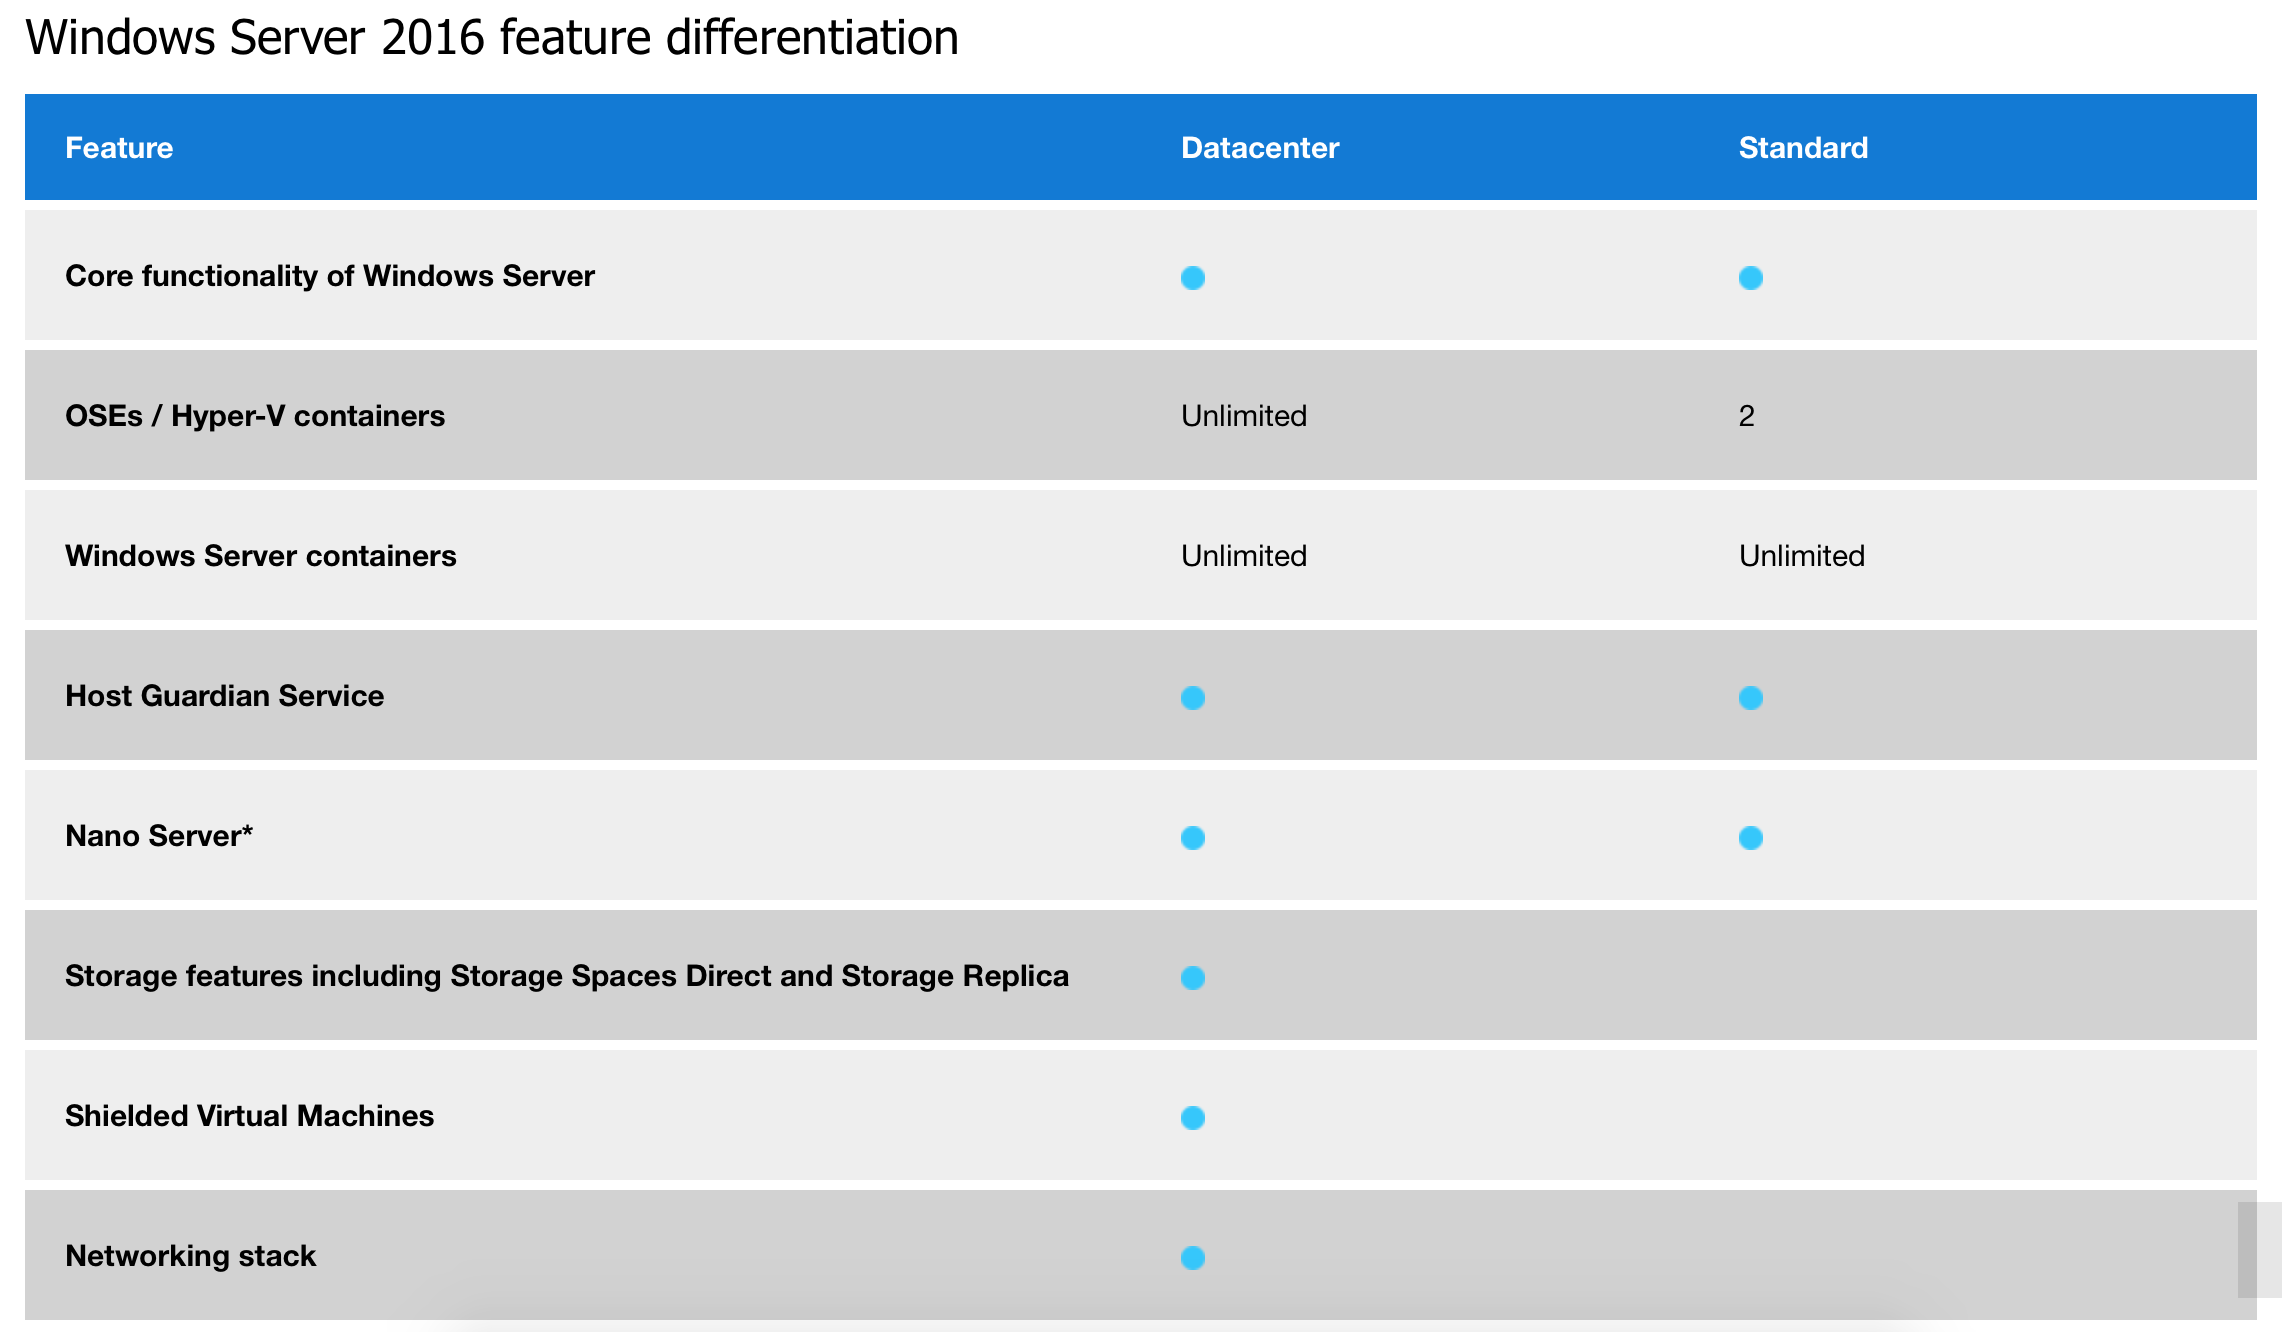
\includegraphics[width=0.7\textwidth]{Imagenes/Diferenciacion_WS2016}
		\caption{Diferencias de características entre WS 2016 Datacenter y WS 2016 Standard.\cite{WS2016DataStandard} } \label{fig:figura10} 
	\end{center}
\end{figure}

%----------------------------------------------------------------------------------------
%	Cuestión 13
%----------------------------------------------------------------------------------------
\section{Continúe usted con el proceso de definición de RAID1 para los dos discos de 50MiB que ha creado. Muestre el proceso con capturas de pantalla.}
\subsection{Respuesta:}
\begin{figure}[H]
	\begin{center}
		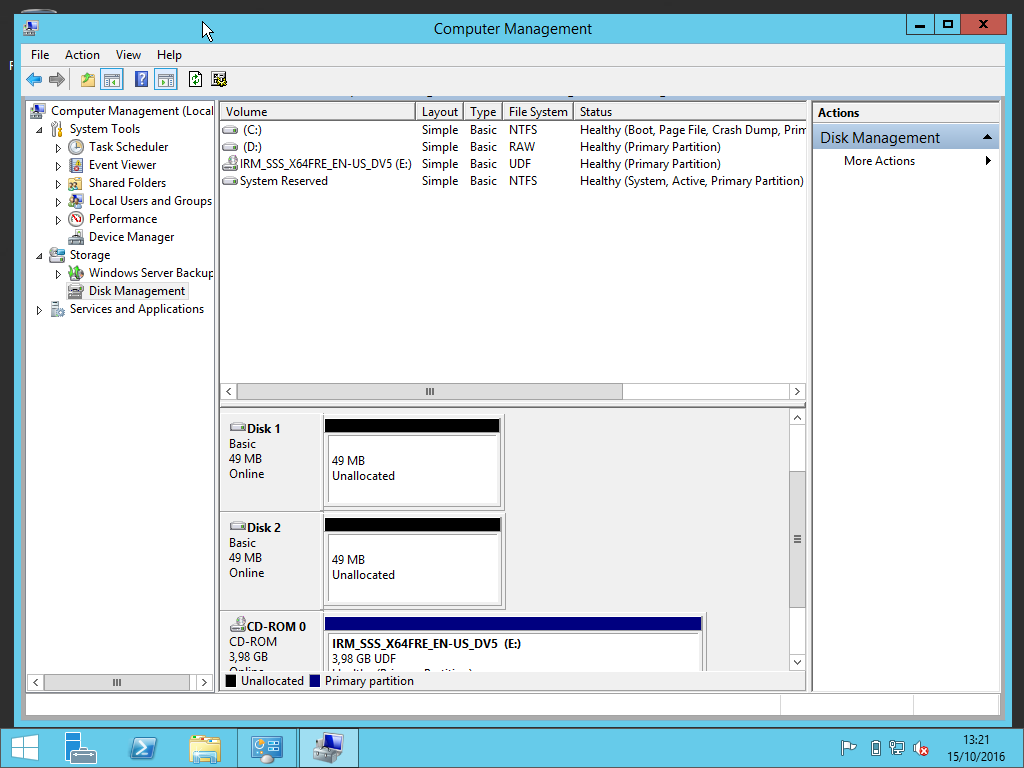
\includegraphics[width=0.7\textwidth]{Imagenes/01_Inicio-configuracion-RAID_1}
		\caption{Entrando a Disk Management para la configuración del volumen reflejado} \label{fig:figura11}
		
		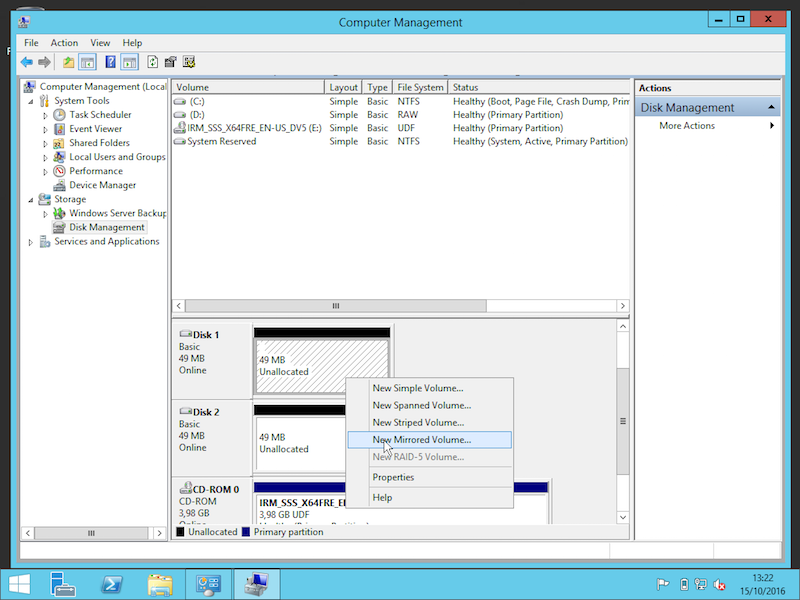
\includegraphics[width=0.7\textwidth]{Imagenes/02_Entrando-a-configurar-volumen-reflejado}
		\caption{Entramos a la configuración, botón derecho sobre el disco a usar como mirrored volume(volumen reflejado)} \label{fig:figura12}
	\end{center}
\end{figure}

\begin{figure}[H]
	\begin{center}
		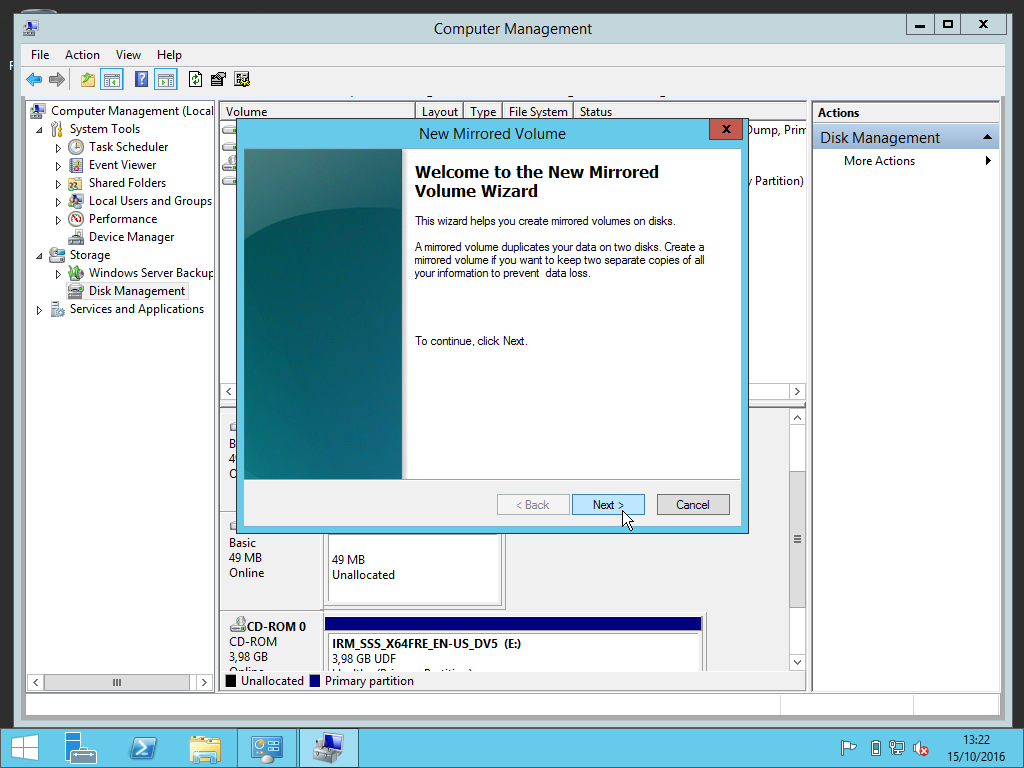
\includegraphics[width=0.7\textwidth]{Imagenes/03_Iniciando-proceso-de-volumen-reflejado}
		\caption{Comienzo del programa para la configuración del volumen reflejado} \label{fig:figura13}
		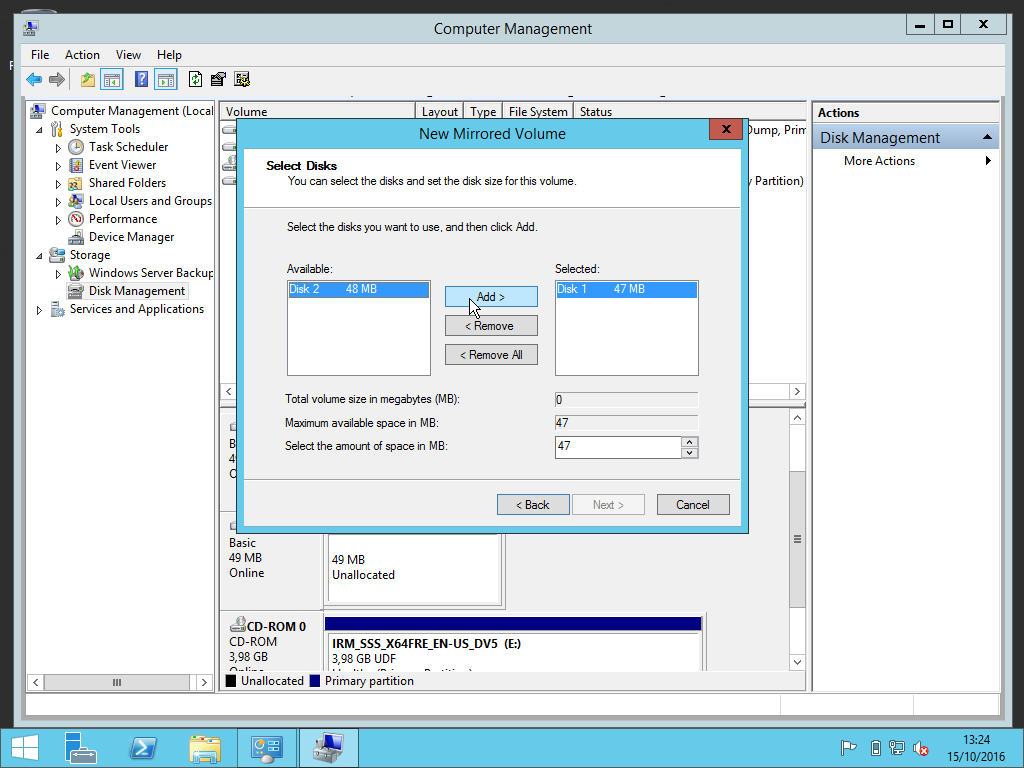
\includegraphics[width=0.7\textwidth]{Imagenes/04_Anadiendo-volumenes-reflejados}
		\caption{Selección de los discos a reflejar, mínimo se necesitan dos} \label{fig:figura14}
	\end{center}
\end{figure}

\begin{figure}[H]
	\begin{center}
		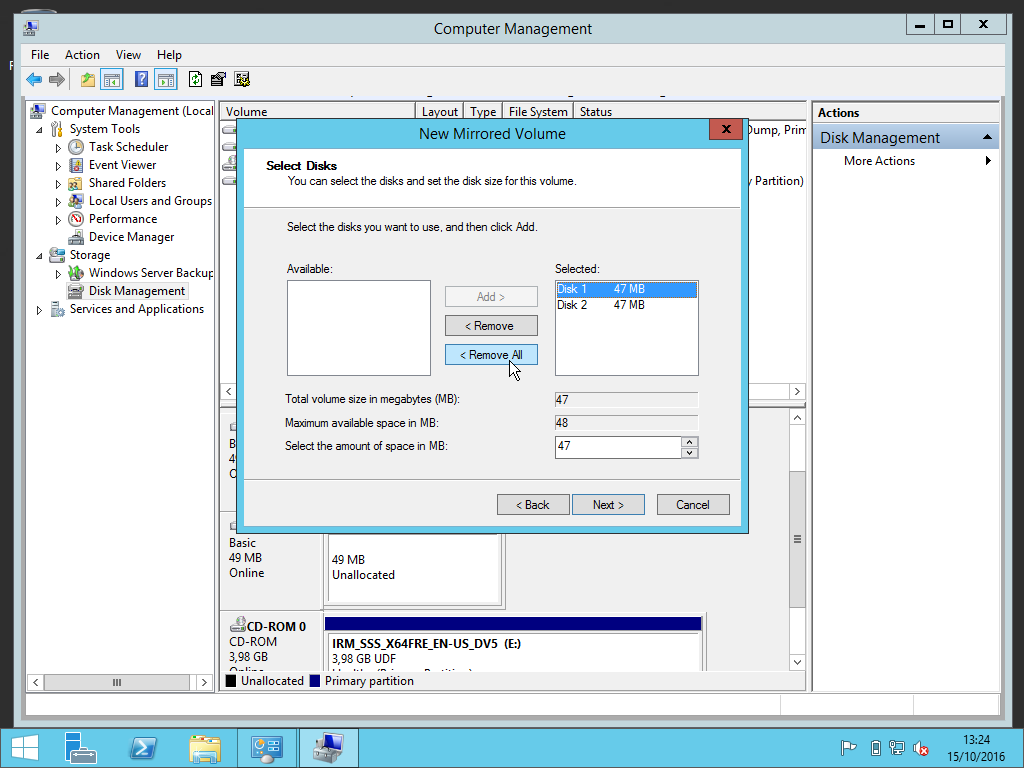
\includegraphics[width=0.7\textwidth]{Imagenes/05_Estado-final-al-anadir-volumenes-reflejados}
		\caption{Ambos discos añadidos para ser reflejados} \label{fig:figura15}
		
		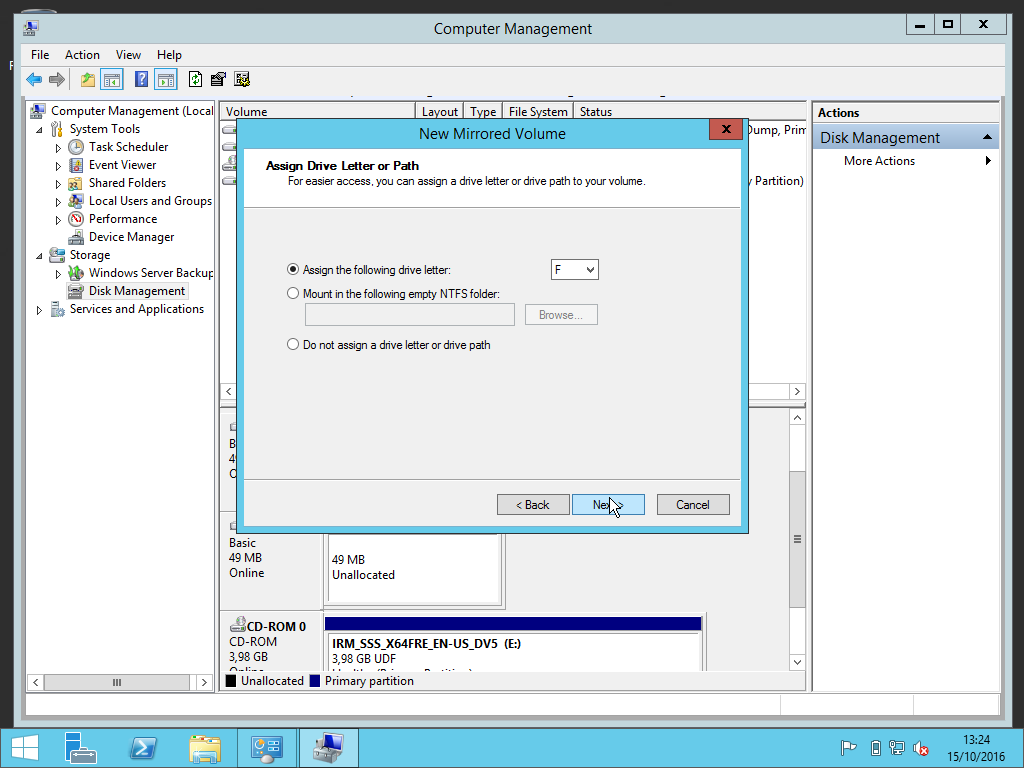
\includegraphics[width=0.7\textwidth]{Imagenes/06_Asignacion-de-letra-al-volumen-final.png}
		\caption{Asignación de letra al volumen} \label{fig:figura16}
	\end{center}
\end{figure}

\begin{figure}[H]
	\begin{center}
		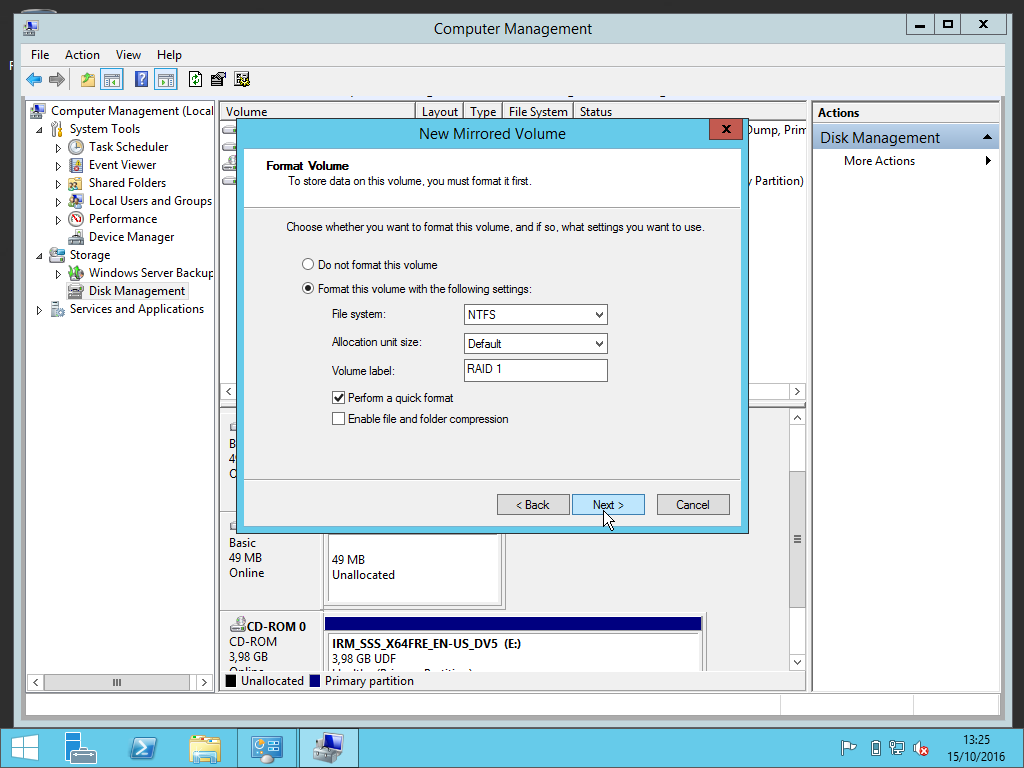
\includegraphics[width=0.7\textwidth]{Imagenes/07_Nombre-del-volumen-y-sistema-de-archivos-final.png}
		\caption{Selección del nombre y sistema de archivos para el volumen} \label{fig:figura17}
		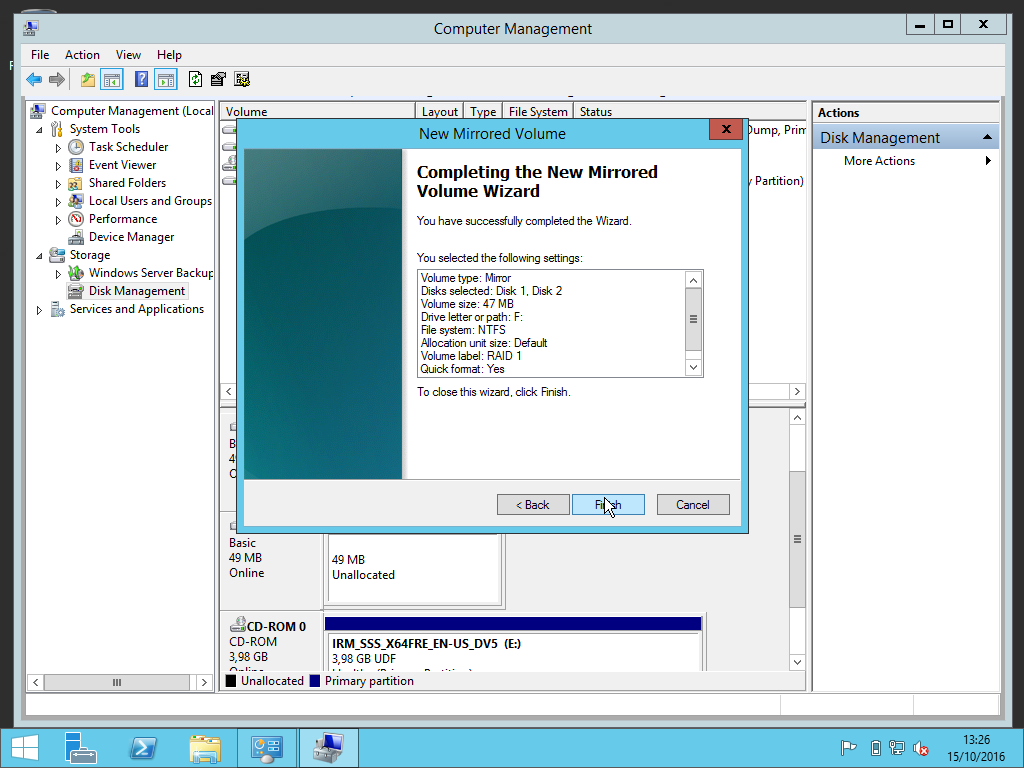
\includegraphics[width=0.7\textwidth]{Imagenes/08_Finalizacion-del-proceso}
		\caption{Finalización del proceso de configuración del volumen reflejado} \label{fig:figura18}
	\end{center}
\end{figure}

\begin{figure}[H]
	\begin{center}
		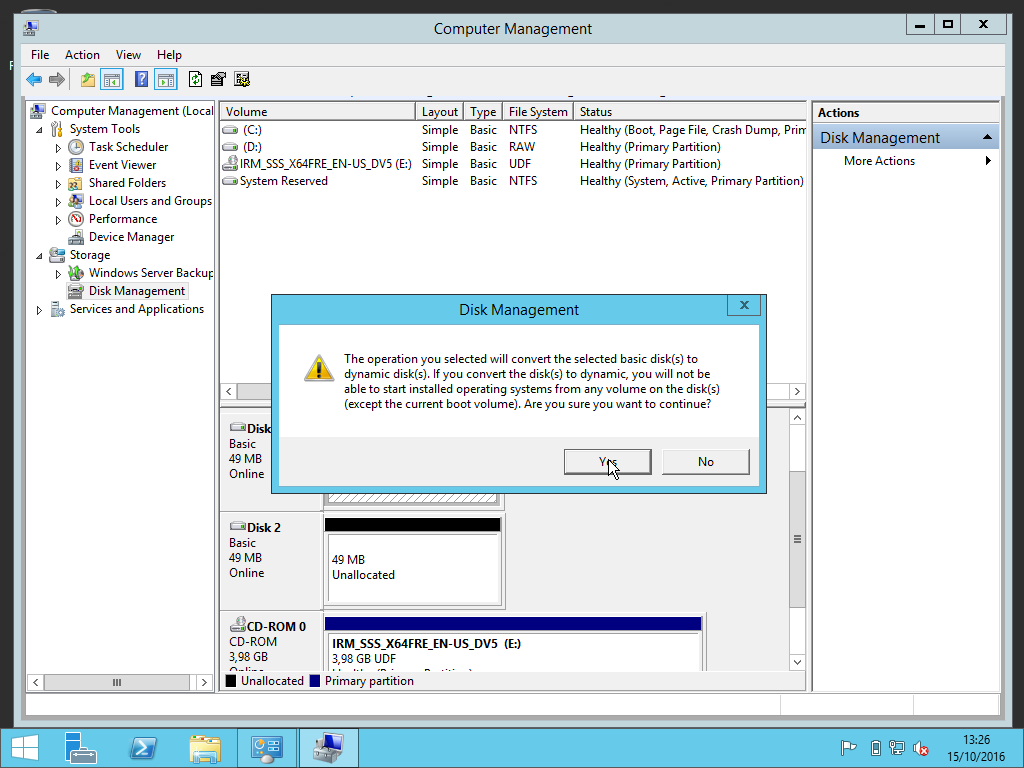
\includegraphics[width=0.7\textwidth]{Imagenes/09_Aceptar-las-modificaciones}
		\caption{Aceptamos las modificaciones que hemos realizado} \label{fig:figura19}
		
		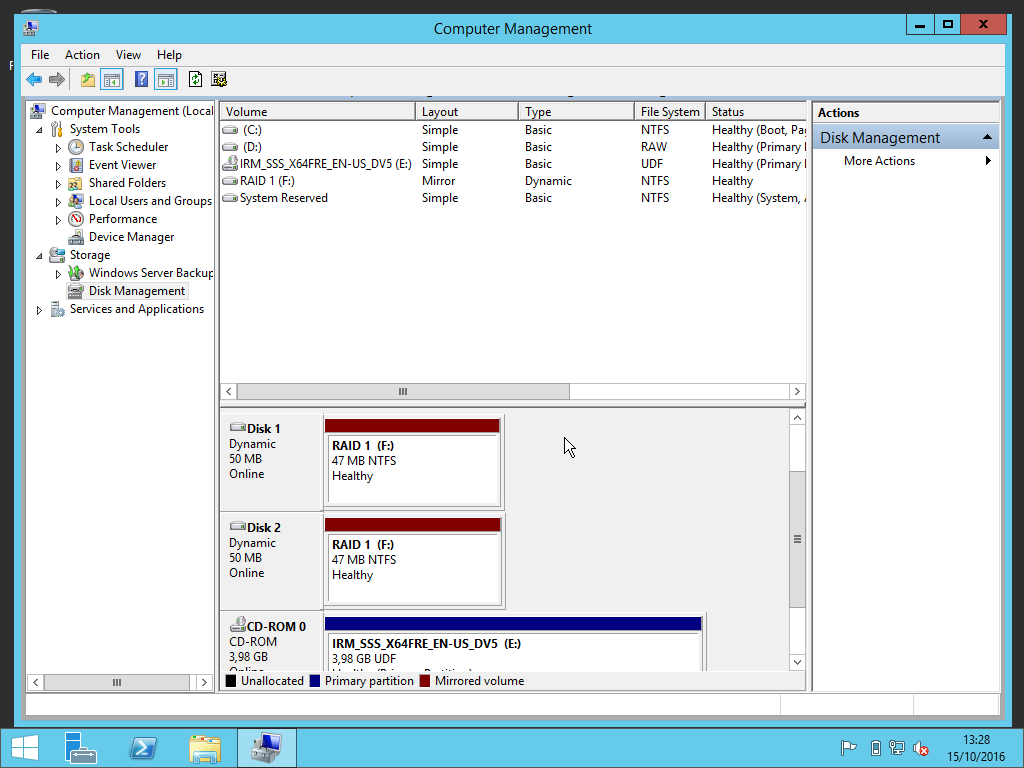
\includegraphics[width=0.7\textwidth]{Imagenes/10_Estado-final-de-ambos-volumenes}
		\caption{Estado final de los discos usados para el RAID} \label{fig:figura20}
	\end{center}
\end{figure}

%----------------------------------------------------------------------------------------
%	Cuestión 14
%----------------------------------------------------------------------------------------
\section{Explique brevemente que diferencias hay entre los tres tipos de conexión que permite el VMSW para las Mvs: NAT, Host-Only y Bridge.}
\subsection{Respuesta:}
\begin{itemize}
	\item NAT: Significa traducción de direcciones de red. Sirve para simplificar y conservar direcciones IP. Este modo permite que la máquina virtual comparta la IP y MAC de la máquina, de tal forma que tienen la misma identidad de red. Este es el modo perfecto para realizar tareas como navegar por internet, descargar archivos y ver el correo electrónico desde el huésped.\cite{ManualVirtualBox} \cite{ManualVMWARE}
	\item Brigde: El modo bridge(puente), hace que la máquina virtual tenga su propia identidad en la red de forma independiente de la máquina. Otros equipos pueden contactar con ella de forma directa. Actúa siendo un equipo más en este aspecto. \cite{ManualVirtualBox} \cite{ManualVMWARE}
	\item Host-Only: En este modo la máquina virtual solamente puede comunicarse con el anfitrión y otras máquinas virtuales en modo host-only. De esta forma la máquina virtual no puede conectarse a internet. Se puede utilizar para proporcionar conectividad entre las máquinas virtuales y el host.
	\cite{ManualVirtualBox} \cite{ManualVMWARE}
\end{itemize}
\newpage
\bibliography{citas} %archivo citas.bib que contiene las entradas 
\bibliographystyle{plain} % hay varias formas de citar

\end{document}
